\documentclass{standalone}
\usepackage{graphicx}	
\usepackage{amssymb, amsmath, amsthm}
\usepackage{color}

\usepackage{tikz}
\usetikzlibrary{intersections, backgrounds, math, decorations.pathreplacing}

\definecolor{light}{RGB}{220, 188, 188}
\definecolor{mid}{RGB}{185, 124, 124}
\definecolor{dark}{RGB}{143, 39, 39}
\definecolor{highlight}{RGB}{180, 31, 180}
\definecolor{darkteal}{RGB}{29, 79, 79}
\definecolor{darkolive}{RGB}{97, 123, 45}
\definecolor{gray10}{gray}{0.1}
\definecolor{gray20}{gray}{0.2}
\definecolor{gray30}{gray}{0.3}
\definecolor{gray40}{gray}{0.4}
\definecolor{gray60}{gray}{0.6}
\definecolor{gray70}{gray}{0.7}
\definecolor{gray80}{gray}{0.8}
\definecolor{gray90}{gray}{0.9}
\definecolor{gray95}{gray}{0.95}

\begin{document}

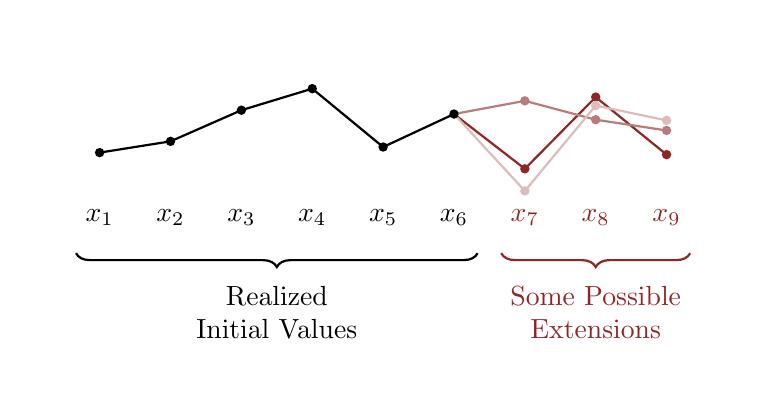
\begin{tikzpicture}[scale=0.3, thick]
  
\draw[white] (0, -7) rectangle (30, 8);
  
 % Possible values
\foreach \n in {7, 8, 9} {
  \node[dark] at ({3 * \n}, 0) { $x_{\n}$ };
}

% Possible realization 1
\foreach \x [count=\n] in {-1.9280710,  1.1094778, -1.3272656} {
  \fill[dark] ({3 * (\n + 6)}, \x + 4) circle (0.2);  
}

\draw[dark] ({3 * 6}, 0.3907344 + 4) \foreach \x [count=\n] in {-1.9280710,  1.1094778, -1.3272656} { -- ({3 * (\n + 6)}, \x + 4) };

%\draw[dark, dashed] (27, -1.3272656 + 4) -- +(3, 0);

% Possible realization 2
\foreach \x [count=\n] in {0.9494158,  0.1507678, -0.3048048} {
  \fill[mid] ({3 * (\n + 6)}, \x + 4) circle (0.2);  
}

\draw[mid] ({3 * 6}, 0.3907344 + 4) \foreach \x [count=\n] in {0.9494158,  0.1507678, -0.3048048} { -- ({3 * (\n + 6)}, \x + 4) };

%\draw[mid, dashed] (27, -0.3048048 + 4) -- +(3, 0);

% Possible realization 3
\foreach \x [count=\n] in {-2.8635426,  0.7495722,  0.1215513} {
  \fill[light] ({3 * (\n + 6)}, \x + 4) circle (0.2);  
}

\draw[light] ({3 * 6}, 0.3907344 + 4) \foreach \x [count=\n] in {-2.8635426,  0.7495722,  0.1215513} { -- ({3 * (\n + 6)}, \x + 4) };

%\draw[light, dashed] (27, 0.1215513 + 4) -- +(3, 0);

% Realized values
\foreach \n in {1, 2, ..., 6} {
  \node at ({3 * \n}, 0) { $x_{\n}$ };
}

%\node[dark] at (30, 0) { $\ldots$ };
  
\foreach \x [count=\n] in {-1.2423804, -0.7652753,  0.5532082,  1.4655993, -1.0053407, 0.3907344} {
  \fill[black] ({3 * \n}, \x + 4) circle (0.2);  
}

\draw[black] (3, -1.2423804 + 4) \foreach \x [count=\n] in {-1.2423804, -0.7652753,  0.5532082,  1.4655993, -1.0053407, 0.3907344} { -- ({3 * \n}, \x + 4) };
 
\draw[decorate,decoration={brace,amplitude=5pt,mirror}] (2, -1.5) -- (19, -1.5);

\node[black,align=center] at (10.5, -4) { Realized\\Initial Values };

\draw[dark, decorate,decoration={brace,amplitude=5pt,mirror}] (20, -1.5) -- (28, -1.5);
  
\node[dark,align=center] at (24, -4) { Some Possible\\Extensions };
  
\end{tikzpicture}

\end{document}  